\chapter{Screenshots}\label{app:screenshots}

\begin{figure}[H]
  \centering
  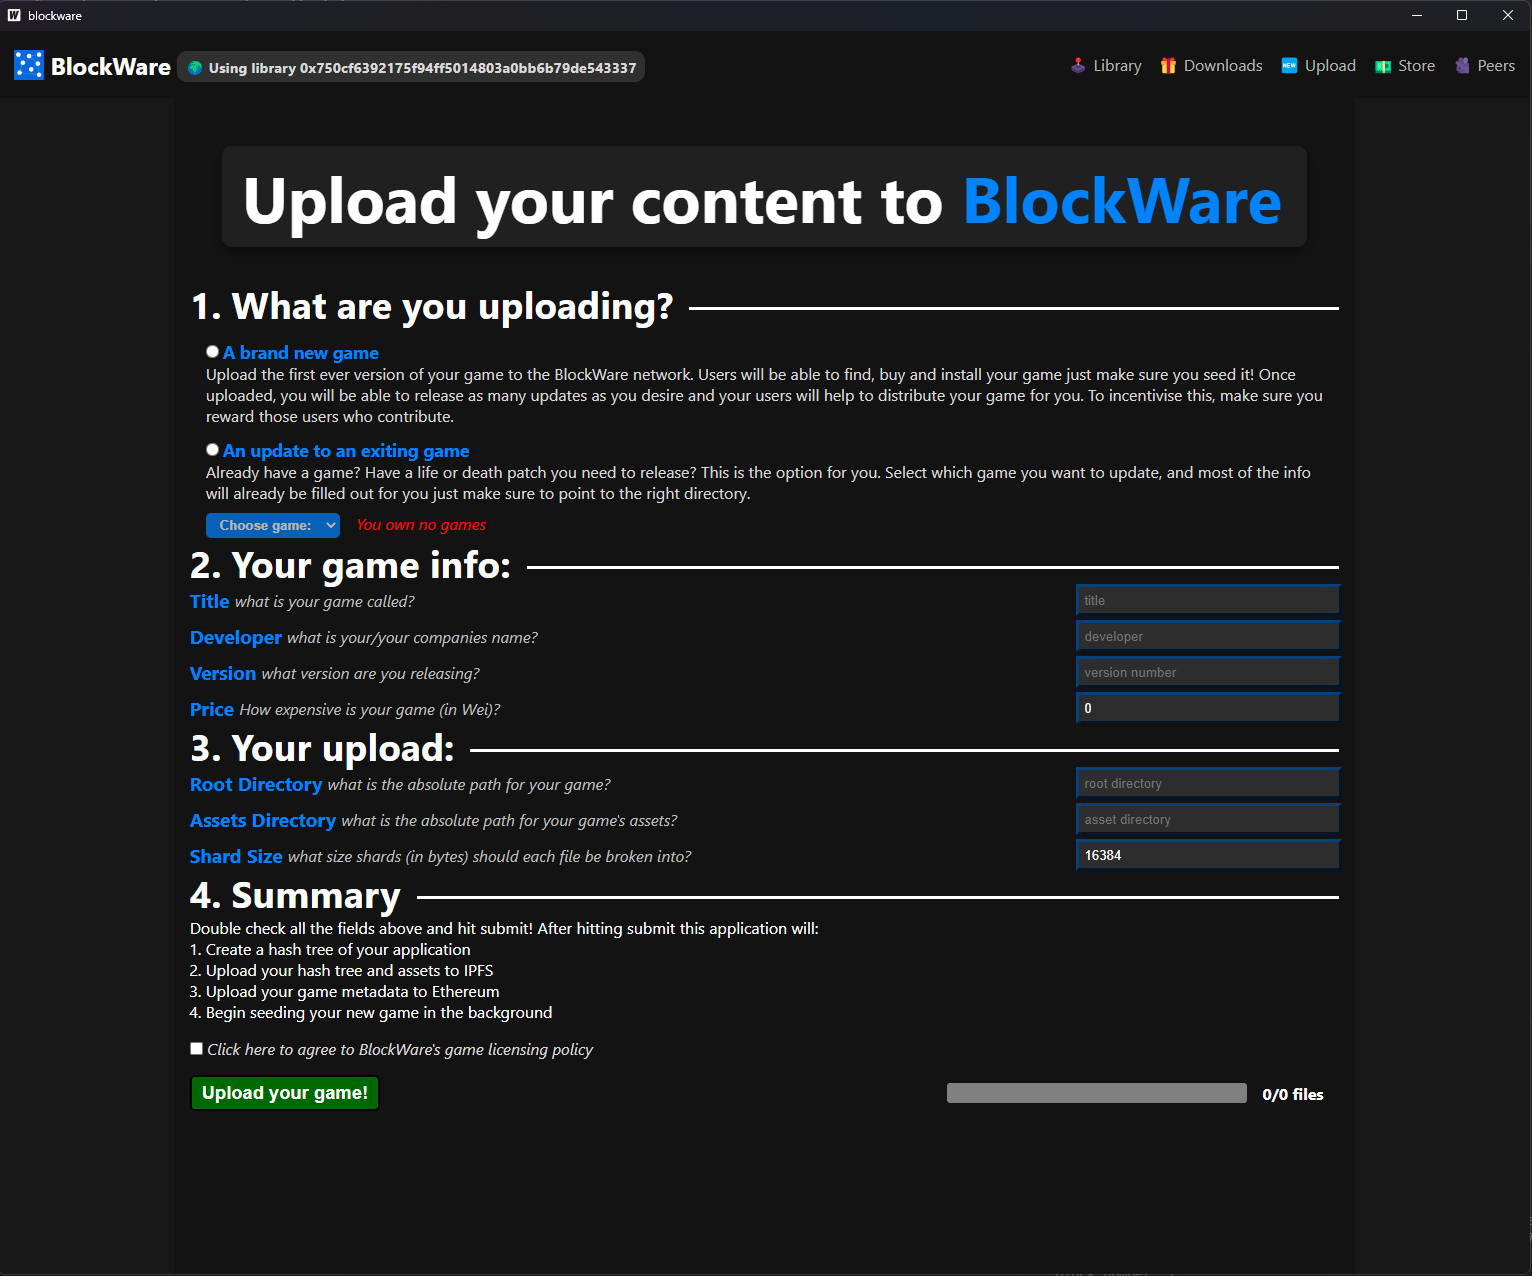
\includegraphics[width=0.9\textwidth]{assets/images/screenshots/upload.png}
  \caption{The page where users input the details about their game and can upload it to the Ethereum network. If a user wants to update a game they can choose from their uploaded games.}
\end{figure}

\begin{figure}[H]
  \centering
  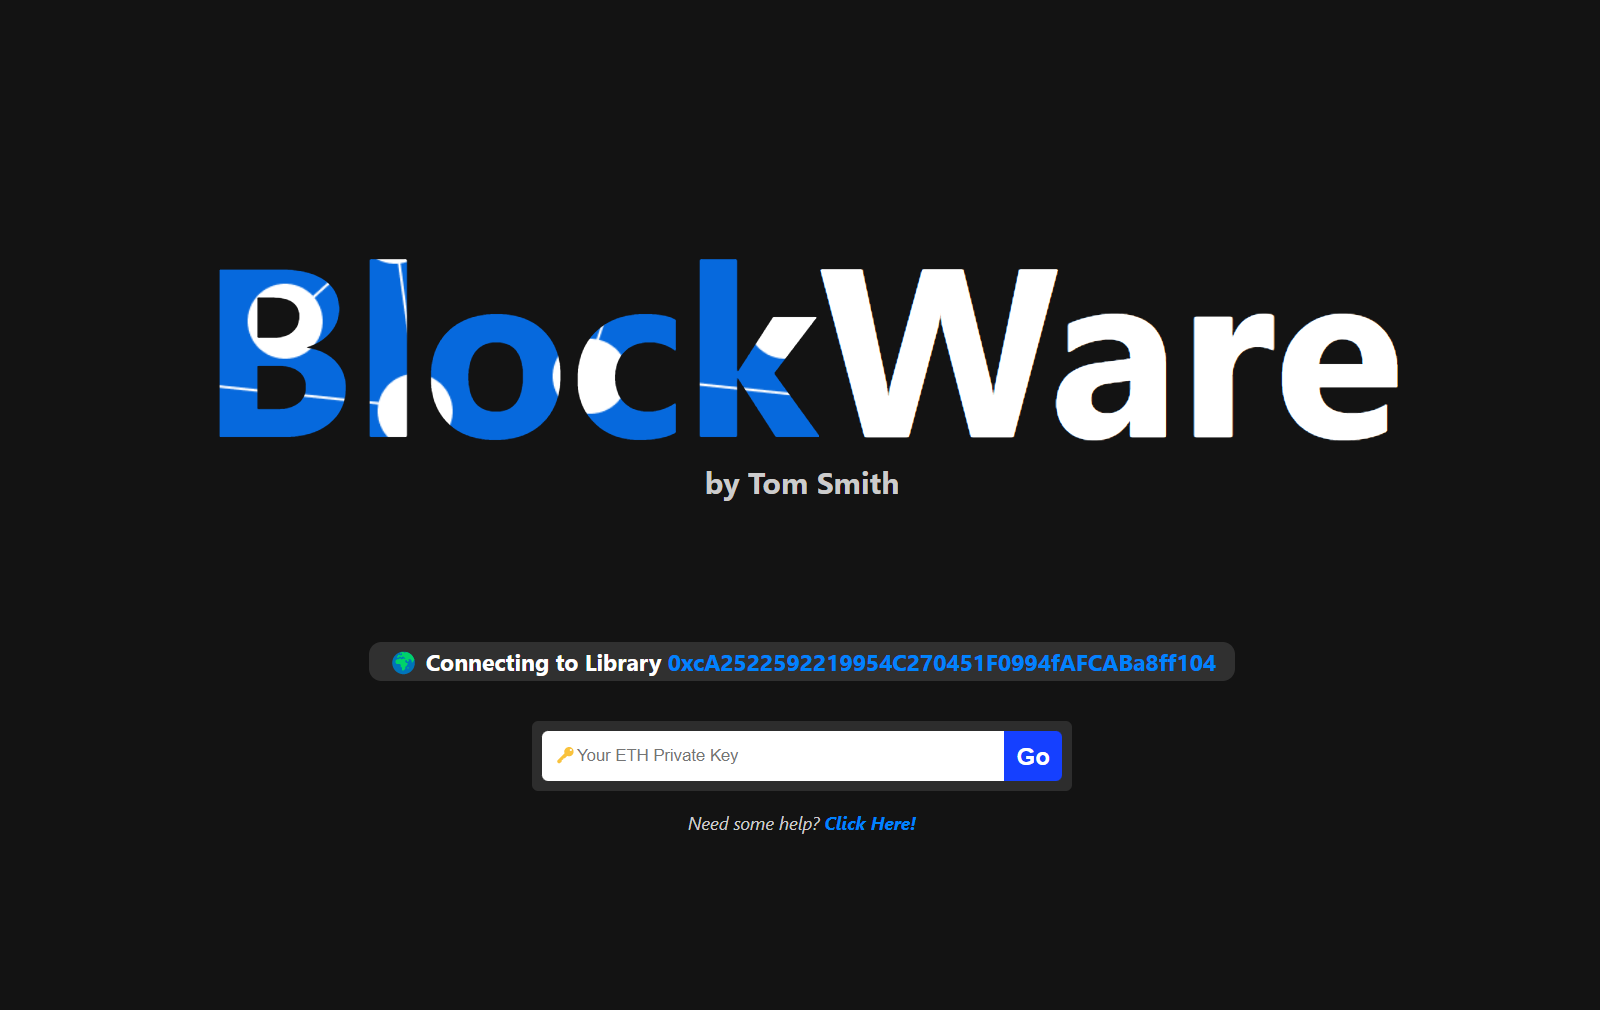
\includegraphics[width=0.9\textwidth]{assets/images/screenshots/login.png}
  \caption{The login page where a user will enter their Ethereum private key and connect to the BlockWare contract instance deployed to Sepolia. Users can access the help page from here.}
\end{figure}

\begin{figure}[H]
  \centering
  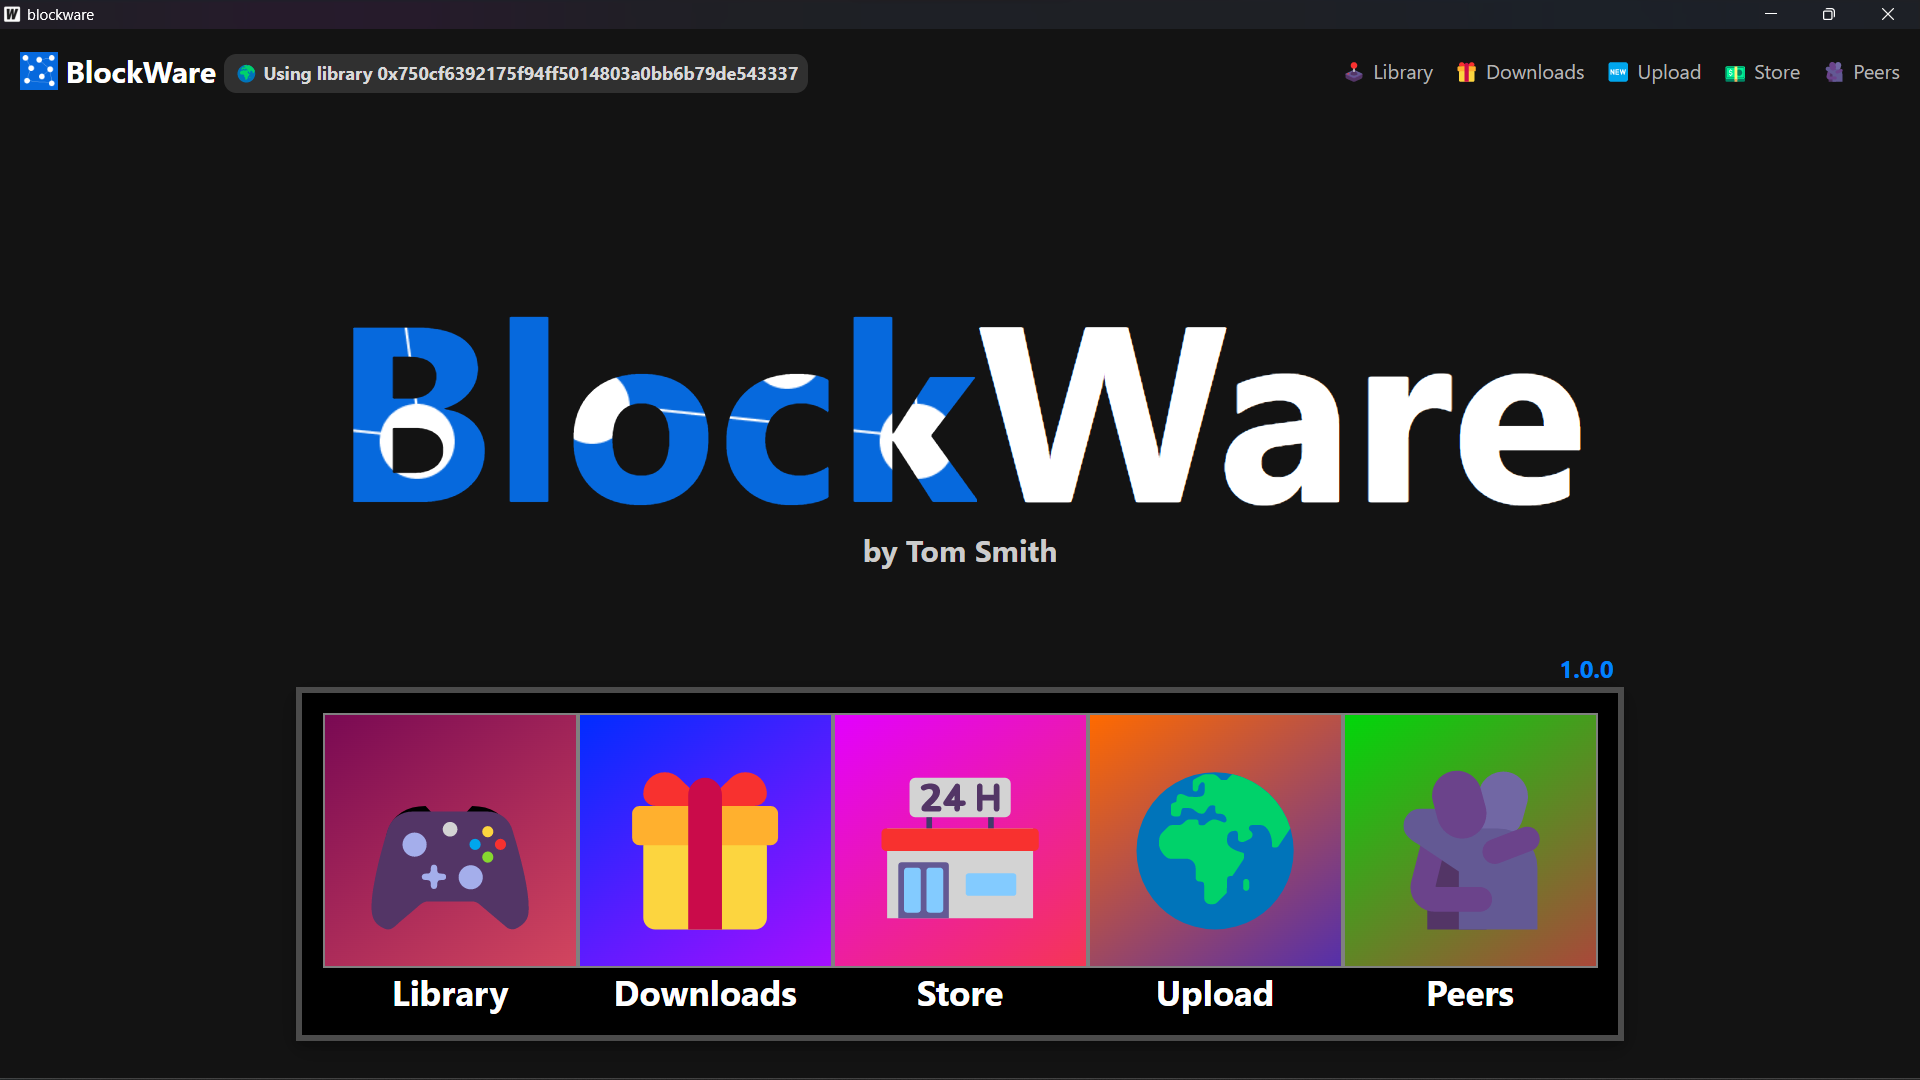
\includegraphics[width=0.9\textwidth]{assets/images/screenshots/home.png}
  \caption{The home page where users can navigate between the main pages.}
\end{figure}

\begin{figure}[H]
  \centering
  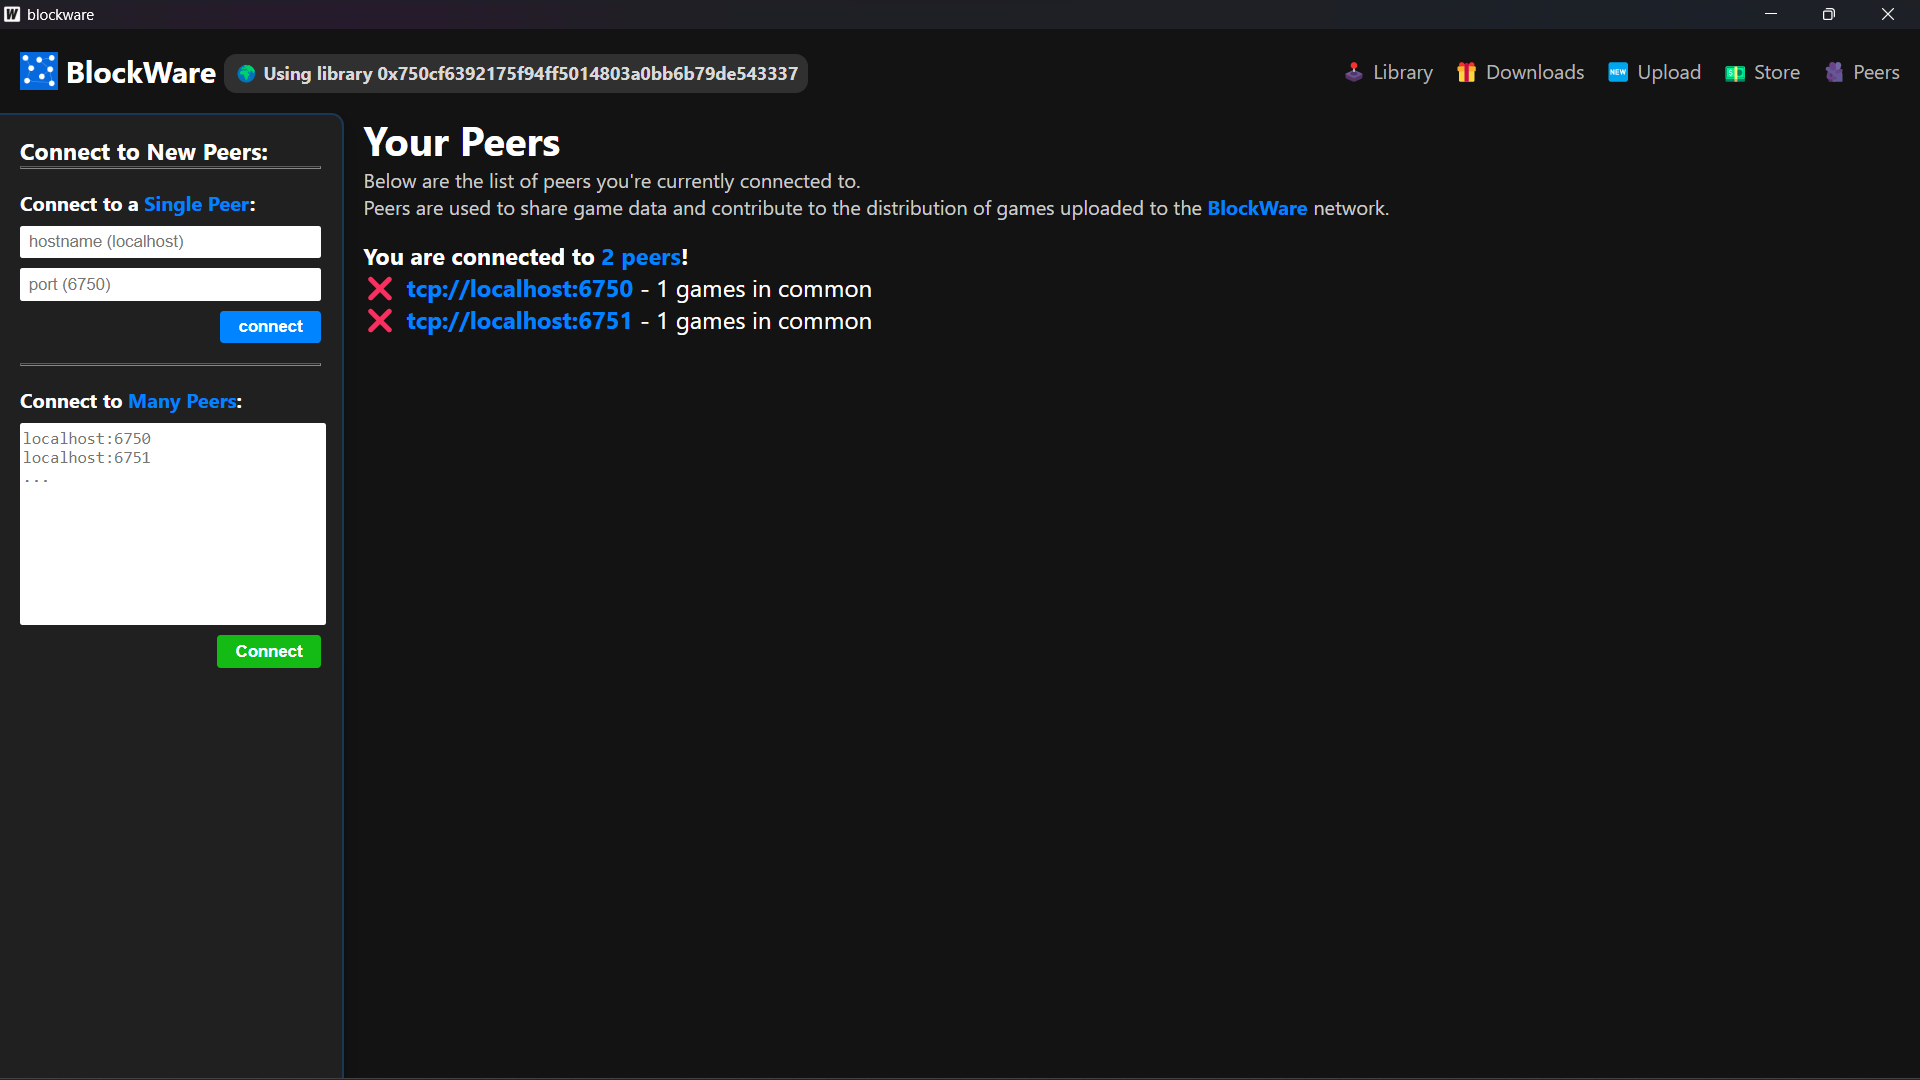
\includegraphics[width=0.9\textwidth]{assets/images/screenshots/peers.png}
  \caption{The page where users can manage their connections to peers with whom they will download game data off of. Users can request receipts from peers that show the amount of data they've sent.}
\end{figure}

\begin{figure}[H]
  \centering
  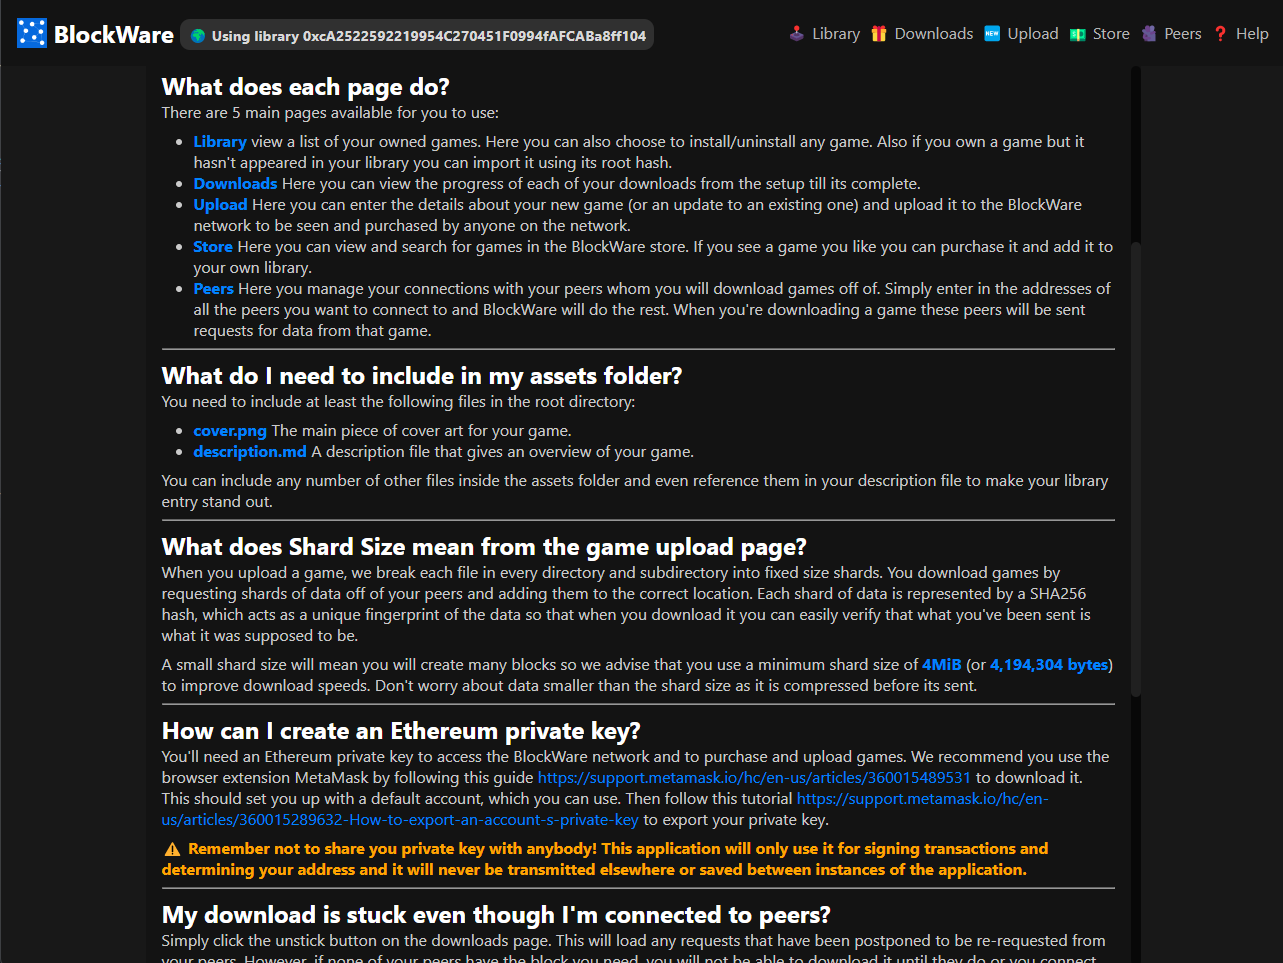
\includegraphics[width=0.9\textwidth]{assets/images/screenshots/help.png}
  \caption{This page has a list of common questions, about the application, expected by users with answers.}
\end{figure}

\begin{figure}[H]
  \centering
  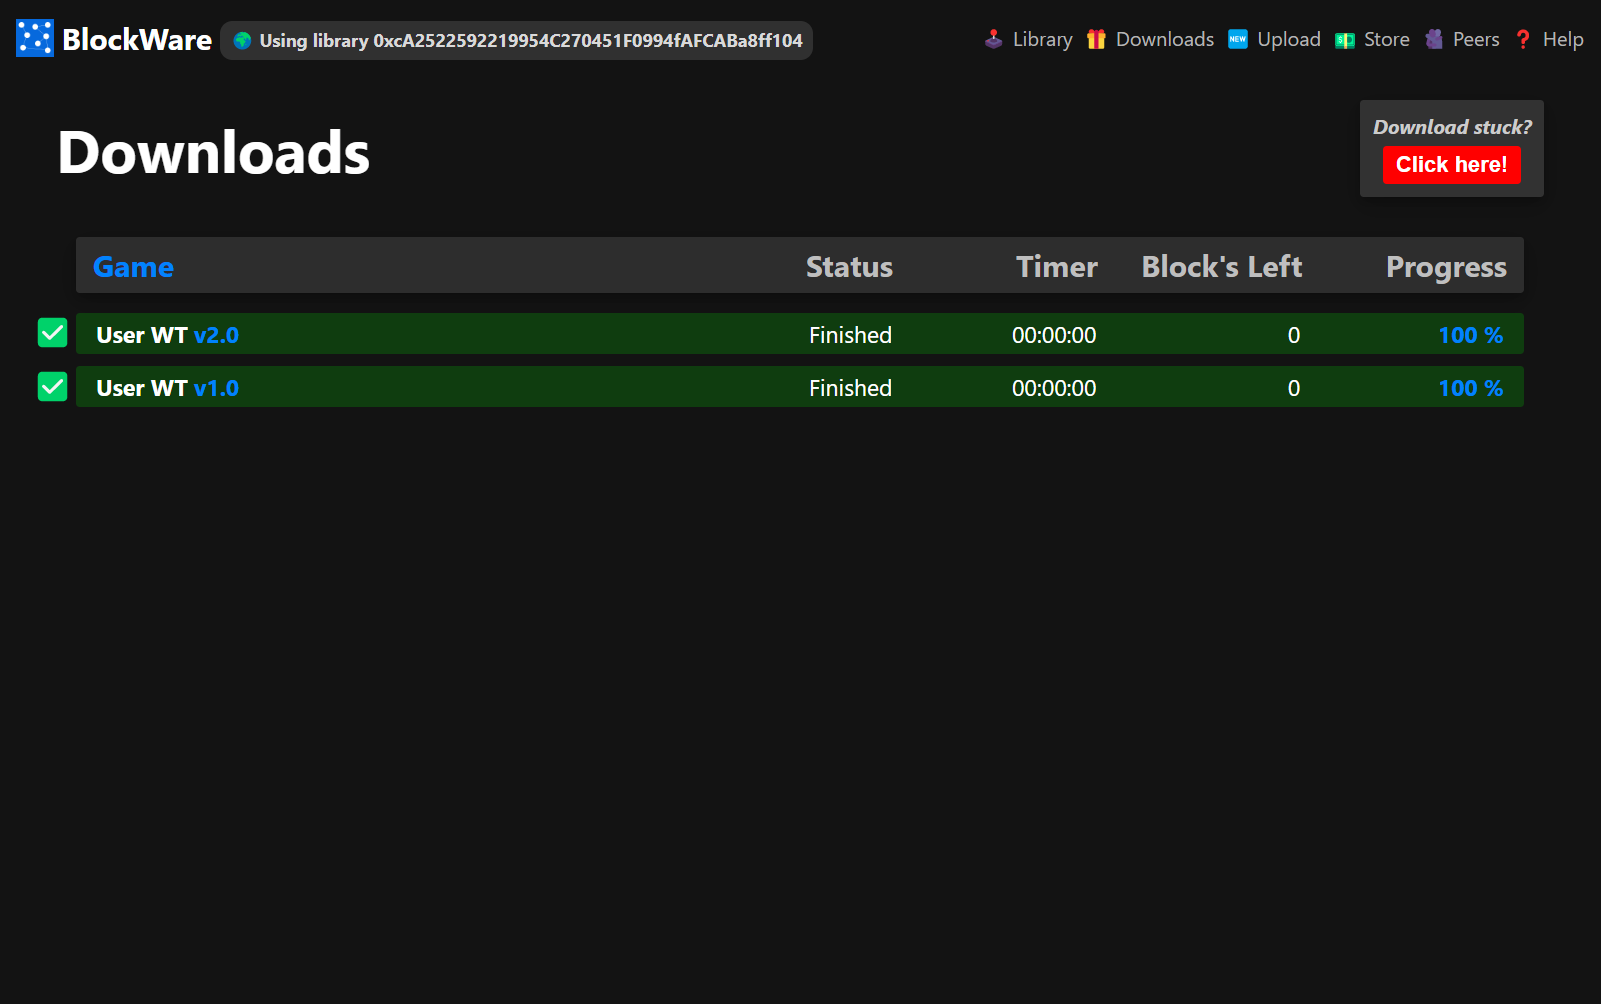
\includegraphics[width=0.9\textwidth]{assets/images/screenshots/downloads.png}
  \caption{This page is where users can track their downloads. It will update in real-time as data is downloaded.}
\end{figure}

\begin{figure}[H]
  \centering
  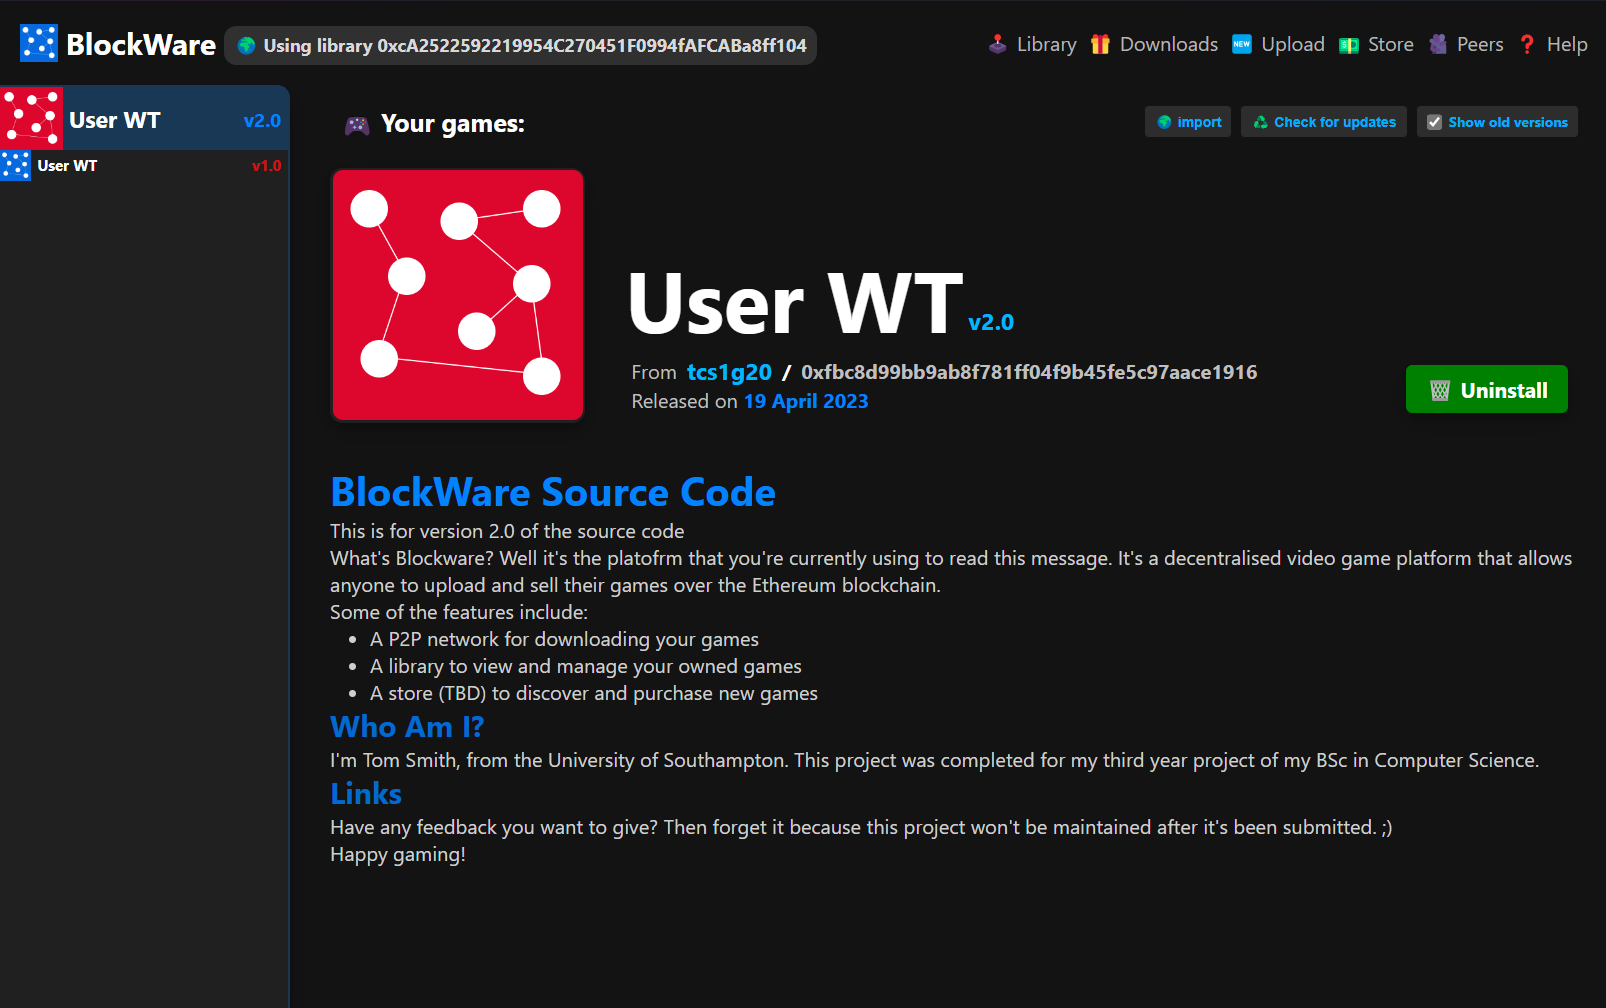
\includegraphics[width=0.9\textwidth]{assets/images/screenshots/library.png}
  \caption{This page shows the user's library of games and allows them to view the assets for them. Smaller games represent older versions of the game and these can be hidden using a the `show old versions' toggle.}
\end{figure}





